\documentclass[10pt,svgnames,usenames,table]{beamer} 

\NeedsTeXFormat{LaTeX2e}

\usetheme[compress]{Singapore} % theme

\usepackage[french]{babel}
\usepackage[T1]{fontenc}
\usepackage[utf8x]{inputenc}
\usepackage{lmodern}
\usepackage{amsmath,amsthm,amssymb}        % un packages mathématiques
\usepackage{pifont}
\newcommand{\cmark}{\ding{51}}%
\newcommand{\xmark}{\ding{55}}%
\usepackage{xcolor}         % pour définir plus de couleurs
\usepackage{graphicx}       % pour insérer des figures
\usepackage{lmodern}
\usepackage{url}
	\urlstyle{sf}
\usepackage{lastpage}
\usepackage{endnotes}

\usepackage{listings}
\usepackage{listingsutf8}

\usepackage{siunitx}
\usepackage{circuitikz}
\usepackage{chemfig}
\usepackage[version=3]{mhchem}

\usepackage[french]{varioref}
\usepackage{wrapfig}
\usepackage{pdfpages}
\usepackage{verbatim}
\usepackage{graphicx}

\usepackage{setspace}

%\usepackage[svgnames]{color}
%\definecolor{webdarkblue}{rgb}{0,0,0.4}
%\definecolor{webgreen}{rgb}{0,0.3,0}
%\definecolor{webblue}{rgb}{0,0,0.8}

\setbeamercolor{section in head/foot}{use=structure,bg=structure.fg!25!bg} % "Amélioration du jeu de couleur"
%\useoutertheme[subsection=true]{smoothbars} % Pour avoir un rappel de la subsection
\setbeamerfont{frametitle}{series=\bfseries}
\setbeamertemplate{frametitle}[default][center] % Titre centré et bien placé.


% "Fioriture de style" : qd <x-> dans les item, les autres en gris clair
\beamertemplatetransparentcovered


% Comportement des itemize
\setbeamertemplate{itemize item}[ball]
\setbeamertemplate{itemize subitem}[triangle]
\setbeamertemplate{itemize subsubitem}[circle]

%\renewcommand\sfdefault{cmss} % Polices

% Les block arrondis et ombrés dans la couleur que je veux
\setbeamertemplate{blocks}[rounded][shadow=true]
\definecolor{normalBlockColor}{RGB}{255,255,255}
\definecolor{normalTitleBlockColor}{RGB}{0,0,102}
\definecolor{normalBlockTextColor}{RGB}{0,0,0}
\definecolor{normalBlockTitleTextColor}{RGB}{255,255,255}
\definecolor{exampleBlockColor}{RGB}{202,251,197}
\definecolor{exampleTitleBlockColor}{RGB}{166,241,158}
\definecolor{exampleBlockTextColor}{RGB}{0,0,0}
\definecolor{exampleBlockTitleTextColor}{RGB}{0,120,0}
\definecolor{alertBlockColor}{RGB}{248,218,218}
\definecolor{alertTitleBlockColor}{RGB}{244,108,108}
\definecolor{alertBlockTextColor}{RGB}{0,0,0}
\definecolor{alertBlockTitleTextColor}{RGB}{120,0,0}
\setbeamercolor*{block title}{fg=normalBlockTitleTextColor,bg=normalTitleBlockColor}
\setbeamercolor*{block body}{fg=normalBlockTextColor,bg=normalBlockColor}
\setbeamercolor*{block title alerted}{fg=alertBlockTitleTextColor,bg=alertTitleBlockColor}
\setbeamercolor*{block body alerted}{fg=alertBlockTextColor,bg=alertBlockColor}
\setbeamercolor*{block title example}{fg=exampleBlockTitleTextColor,bg=exampleTitleBlockColor}
\setbeamercolor*{block body example}{fg=exampleBlockTextColor,bg=exampleBlockColor}
\setbeamerfont{block title}{size={}}



%------------ fin style beamer -------------------

% Faire apparaître un sommaire avant chaque section
% \AtBeginSection[]{
%   \begin{frame}
%   \frametitle{Plan}
%   \medskip
%   %%% affiche en début de chaque section, les noms de sections et
%   %%% noms de sous-sections de la section en cours.
%   \small \tableofcontents[currentsection, hideothersubsections]
%   \end{frame}
% }


% Pour personnaliser la barre de navigation du dessous
\setbeamertemplate{navigation symbols}{
	%\insertslidenavigationsymbol
	%\insertframenavigationsymbol
	%\insertsubsectionnavigationsymbol
	\quad\textbf{\insertframenumber/\inserttotalframenumber} % Numéro de page
	%\insertsectionnavigationsymbol
	%\insertdocnavigationsymbol
	%\insertbackfindforwardnavigationsymbol
}
% Supprimer les icones de navigation (pour les transparents)
%\setbeamertemplate{navigation symbols}{}

% Mettre les icones de navigation en mode vertical (pour projection)
% \setbeamertemplate{navigation symbols}[vertical]

\newenvironment{itemize2}%
	{ \begin{list}%
		{$\bullet$}%
		{\setlength{\labelwidth}{30pt}%
		 \setlength{\leftmargin}{35pt}%
		 \setlength{\itemsep}{\parsep}}}%
	{ \end{list} }

\def\siecle#1{\textsc{\romannumeral #1}\textsuperscript{e}~siècle} % => le \siecle{19}

\definecolor{codeBlue}{rgb}{0,0,1}
\definecolor{webred}{rgb}{0.5,0,0}
\definecolor{codeGreen}{rgb}{0,0.5,0}
\definecolor{codeGrey}{rgb}{0.6,0.6,0.6}
\definecolor{webdarkblue}{rgb}{0,0,0.4}
\definecolor{webgreen}{rgb}{0,0.3,0}
\definecolor{webblue}{rgb}{0,0,0.8}
\definecolor{orange}{rgb}{0.7,0.1,0.1}
\lstset{
      language=TeX,
      flexiblecolumns=true,
      numbers=left,
      stepnumber=1,
      numberstyle=\ttfamily\tiny,
      keywordstyle=\ttfamily\textcolor{blue},
      stringstyle=\ttfamily\textcolor{red},
      commentstyle=\ttfamily\textcolor{codeGreen},
      breaklines=true,
      extendedchars=true,
      basicstyle=\ttfamily\scriptsize,
      showstringspaces=false,
      morekeywords={usepackage,documentclass,begin,textbf,textit,texttt,ref,includegraphics,caption,label,setlength,mathbb,notag,frac,num,si,ang,SI,textwidth,percent,meter,ohm,joule,second,more,section,subsection,tableofcontents,setstretch,TeX,LaTeX,huge,sffamily,emph,chemfig,pageref,vpageref,date,maketitle,institute,author,and,textsc,title,includeonly,include,clearpage,newcommand,mathsf,renewcommand,DeclareMathOperator,mathrm,captionof,lstinputlisting,lstinline},
      frame=single,
      extendedchars=true,
      inputencoding=utf8x,
	    literate={á}{{\'a}}1 {ã}{{\~a}}1 {é}{{\'e}}1 {è}{{\`e}}1 {à}{{\`a }}1
    }
\lstset{inputencoding=utf8/latin1}

\newsavebox\mybox
\newenvironment{aquote}[1]
{\savebox\mybox{#1}\begin{quote}}
{{{\leavevmode\unskip\nobreak\hfil\penalty50\hskip2em
    \hbox{}\nobreak\hfil(\usebox\mybox)%
\parfillskip=0pt \finalhyphendemerits=0 \endgraf}}\end{quote}}

%\setbeamertemplate{headline}{}

\usepackage{pdflscape} %% portrait
\usepackage[french]{varioref} % \vpageref
\usepackage{pgfplots}
\usepackage{framed}
\usepackage{mdframed}
\usepackage{epstopdf}
\usepackage{xspace}
\usepackage{caption}
\usepackage{menukeys}
\captionsetup[figure]{labelformat=empty}

\usepackage[colorinlistoftodos]{todonotes}%disable=true

\newcommand{\badet}{et}
\newcommand{\goodet}{\mathbin{\mathrm{et}}}
\DeclareMathOperator{\sumN}{\sum_{i=1}^n}
\DeclareMathOperator{\var}{\mathrm{Var}}

\lstdefinestyle{nonumbers}
{numbers=none}

% Pour rendre les toc plus compactes (pour éviter que ça déborde)
\makeatletter
\patchcmd{\beamer@sectionintoc}{\vskip1.5em}{\vskip0.5em}{}{}
\makeatother
\setbeamerfont{subsection in toc}{size=\scriptsize}

\graphicspath{{Images/}}
\definecolor{gris}{RGB}{228,228,228}
\definecolor{bleu}{RGB}{34,148,255}
\definecolor{darkgray}{rgb}{0.3,0.3,0.3}
\usefonttheme[onlymath]{serif} % to see the difference when I do mathsf

\logo{
\includegraphics[height=5mm]{logo_12-13-mini.png}}
\institute{Louvain-li-Nux}
\title{\textbf{Formation GIMP}\\
Introduction au montage photo avec GIMP}
\author{Adrien~\textsc{Couplet} \and Sébastien~\textsc{de Longueville} \and Laurent~\textsc{Ziegler}}

\date{5 avril 2018}


\begin{document}

\begin{frame}
	\maketitle
\end{frame}

\begin{frame}
  \begin{center}\Large
  Suivez cette présentation sur votre ordinateur :-)
  
  \vspace{1cm}
  \fbox{\url{https://louvainlinux.org/activites/atelier-gimp}}
  \end{center}
\end{frame}

\section{Introduction}
\begin{frame}[allowframebreaks]{Qu'est-ce que GIMP ?}
    \begin{itemize}
        \item GIMP = GNU Image Manipulation Program
        \item Logiciel de traitement d'images bitmap.
        \item Alternative gratuite et libre à Adobe Photoshop
    \end{itemize}
    \begin{figure}
        \centering
        
\includegraphics[width=0.5\textwidth]{Images/gimp-logo.png}
        \caption{Wilber, la mascotte officielle de GIMP} 
    \end{figure}
    \framebreak
    Liste non exhaustive des fonctionnalités de GIMP
    \begin{itemize}
        \item Gestion des calques;
        \item Plusieurs outils de dessin;
        \item Plusieurs outils de sélection;
        \item Outils de transformation;
        \item Une sélection de filtres;
        \item Gestion de nombreux formats (JPEG, GIF, PNG, PSD, TIFF);
        \item ...
    \end{itemize}
\end{frame}

\begin{frame}{Installation}
    \begin{center}
    GIMP est disponible pour Windows, Linux et macOS
    \vspace{1cm}\Large
    \fbox{\url{https://www.gimp.org/downloads/}}
    \end{center}
\end{frame}

\section{Présentation de l'interface et des outils}
\begin{frame}[allowframebreaks]{L'interface}
    \begin{figure}
        \centering
        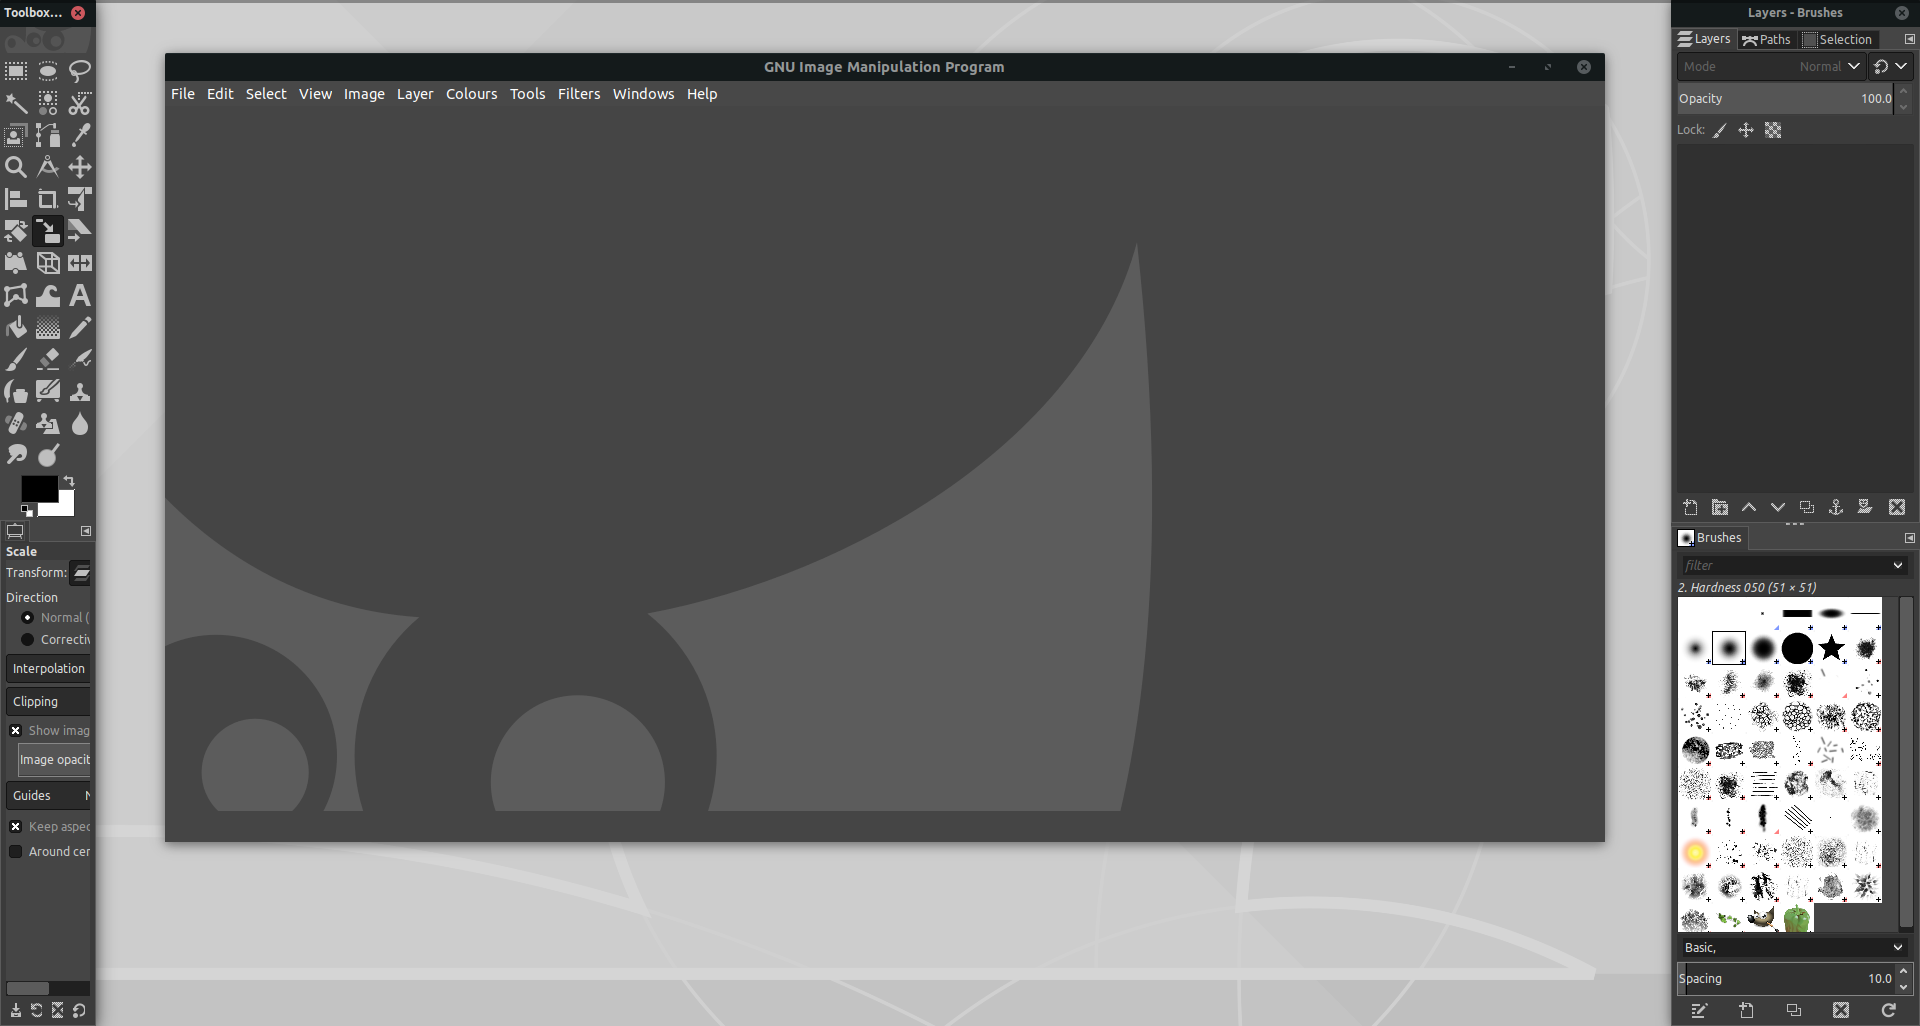
\includegraphics[width=0.9\textwidth]{Images/gimp_multiple_windows.png}
        \caption{L'interface multi-fenêtres}
    \end{figure} 
    \framebreak
    \begin{center}
        Fenêtres > Mode fenêtre unique
        \begin{figure}
            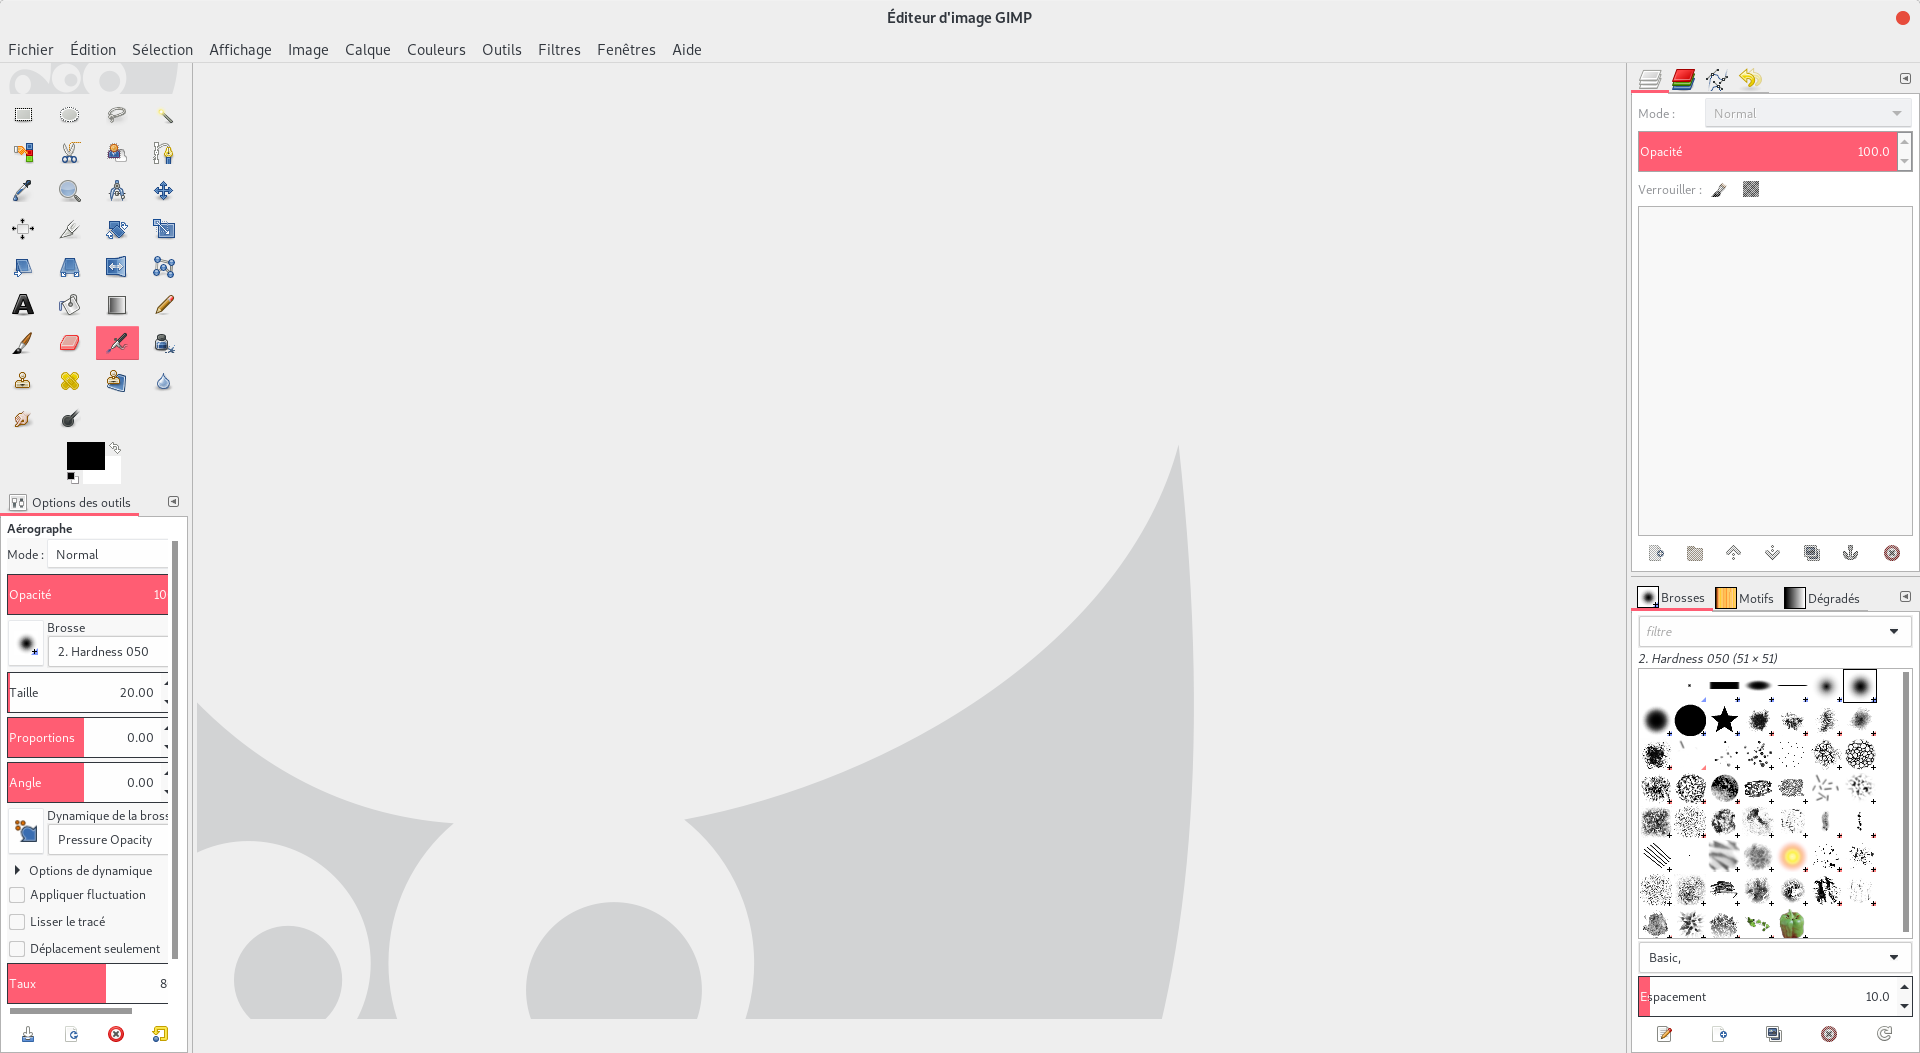
\includegraphics[width=0.9\textwidth]{Images/gimp_single_window.png}
            \caption{L'interface fenêtre unique}
        \end{figure}
    \end{center}
\end{frame}

\begin{frame}{Créer/importer une image}
	\begin{itemize}
		\item Pour \textbf{créer} une image: Fichier > Nouvelle image ou \keys{\ctrl + N}
			\begin{itemize}
				\item Sélectionnez un modèle (A3, A4, A5...) ou spécifier manuellement les dimensions (en pixels, mm, cm...).
			\end{itemize}
		\item Pour \textbf{importer} une image: Fichier  > Ouvrir ou \keys{\ctrl + O}.
			\begin{itemize}
				\item GIMP supporte de nombreux formats: PNG, JPEG, GIF...
			\end{itemize}
		\item Pour \textbf{créer} depuis le presse-papiers (copier/coller): Créer > Depuis le presse-papiers ou \keys{\shift + \ctrl + V}
	\end{itemize}
	\begin{center}
		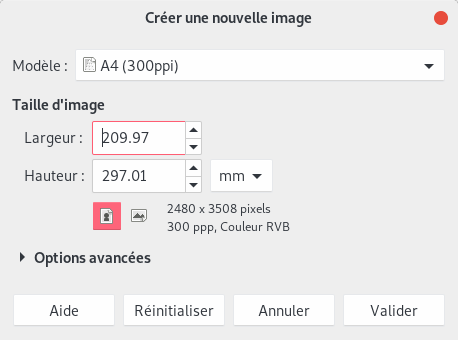
\includegraphics[width=0.5\textwidth]{Images/new_image.png}
	\end{center}
\end{frame}

\begin{frame}{Une image c'est quoi ?}
	\begin{center} 
		\textbf{Image matricielle} $\leftrightarrow$ Image vectorielle 
		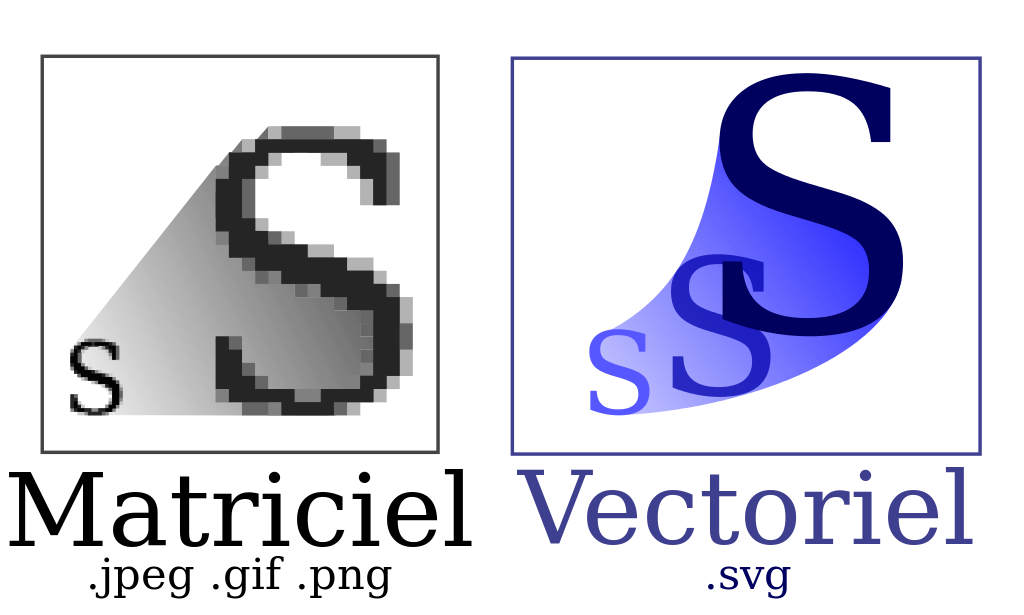
\includegraphics[width=0.6\textwidth]{Images/mat_vs_vec.png}
	\end{center}
	Pourquoi on utilise pas toujours des images vectorielles ? 
	\begin{itemize}
		\item les images vectorielles ne peuvent afficher que des images construites à l'aide de formes. Les images matricielles ont l'avantage d'être définies au pixel près.
	\end{itemize}
\end{frame}

\begin{frame}{Les formats}
	Stocker chaque pixel demande beaucoup de mémoire. Solution ? Compresser les images:
	\begin{itemize}
		\item compression sans pertes (PNG, GIF);
		\item compression avec pertes (JPEG).
	\end{itemize}
	Les trois principaux formats d'images sont
	\begin{itemize}
		\item \textbf{JPEG}: léger (mais avec pertes), idéal pour les photos;
		\item \textbf{PNG}: plus lourd que JPEG (mais sans pertes), très bon support de la transparence;
		\item \textbf{GIF}: support des animations, limité à 256 couleurs.
	\end{itemize}
	Un projet GIMP sera sauvegardé au format \textbf{XCF}, un format d'image libre qui contiendra les différents calques et paramètres de votre création.
	
	L'équivalent d'Adobe Photoshop est le format \textbf{PSD}.
\end{frame}

\begin{frame}{Enregistrement et exportation}
	\begin{itemize}
		\item Pour \textbf{enregistrer} au format \textbf{XCF}: Fichier > Enregistrer ou \keys{\ctrl + S}.
		\item Pour \textbf{exporter} votre image dans un autre format: Fichier > Exporter ou \keys{\shift + \ctrl + E}.
	\end{itemize}
	\begin{center}
		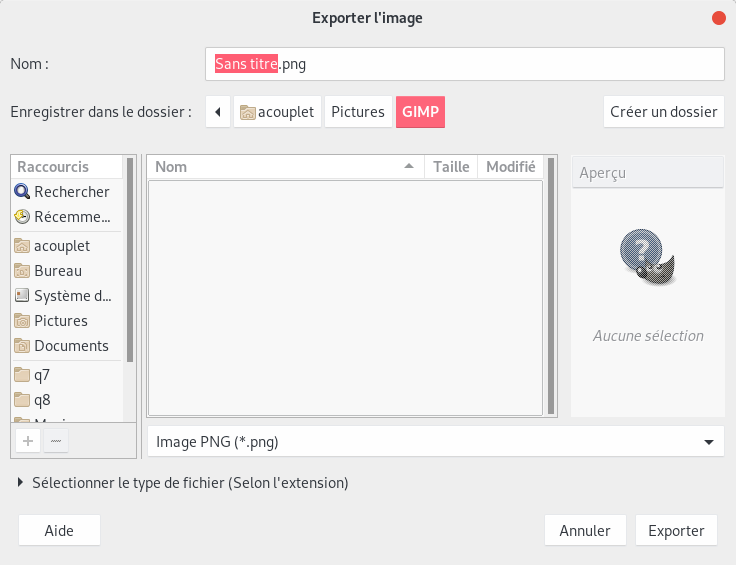
\includegraphics[width=0.5\textwidth]{Images/export.png}
	\end{center}
\end{frame}

\begin{frame}{Les couleurs}
	Il est possible de gérer 2 couleurs: les couleurs de premier et d'arrière-plan:
	\begin{center}
		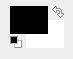
\includegraphics[width=0.08\textwidth]{Images/color_primary.png}
	\end{center}
	Il suffit de cliquer sur une de ces couleurs pour la modifier:
	\begin{center}
		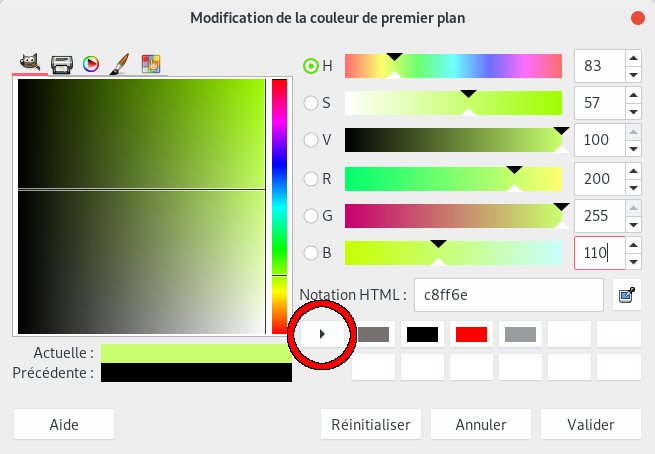
\includegraphics[width=0.5\textwidth]{Images/color_selector.png}
	\end{center}
	Il est possible de sélectionner une couleur ou de rentrer ses valeurs RGB. Une fois votre couleur choisie, vous pouvez l'ajouter à votre palette.
\end{frame}

\begin{frame}[allowframebreaks]{Les outils de coloration}
	La \textbf{pipette} permet de récupérer la couleur d'un pixel d'une image en cliquant sur le pixel en question.
	\begin{center}
		
\includegraphics[width=0.05\textwidth]{Images/color_tool_0.png}
		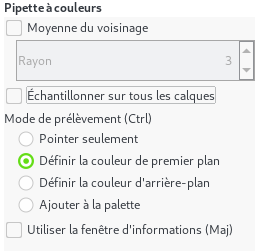
\includegraphics[width=0.3\textwidth]{Images/color_tool_0_settings.png}
	\end{center}
	L'outil permet de définir la couleur de premier plan, la couleur d'arrière-plan ou simplement d'ajouter la couleur à la palette.
	
	\framebreak
	Le \textbf{pot de peinture} permet de remplir une zone.
	\begin{center}
		
\includegraphics[width=0.05\textwidth]{Images/color_tool_1.png}
		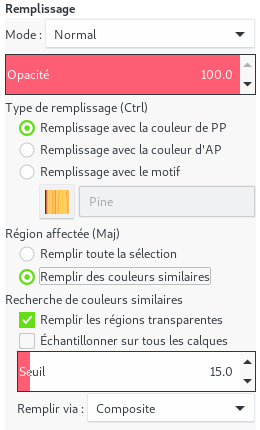
\includegraphics[width=0.25\textwidth]{Images/color_tool_1_settings.png}
	\end{center}
	Le seuil permet d'ajuster la zone à remplir: 
	\begin{center}
		
\includegraphics[width=0.3\textwidth]{Images/color_tool_1_test0.png}
		
\includegraphics[width=0.3\textwidth]{Images/color_tool_1_test1.png}
		
\includegraphics[width=0.3\textwidth]{Images/color_tool_1_test2.png}
	\end{center}
	\begin{scriptsize}
	Exemple: image originale, remplissage noir avec seuil à 30, remplissage noir avec seuil à 60.
	\end{scriptsize}
	
	\framebreak
	L'outil de gradient permet de créer des dégradés entre la couleur de premier plan et celle d'arrière-plan.
	\begin{center}
		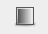
\includegraphics[width=0.05\textwidth]{Images/color_tool_2.png}
		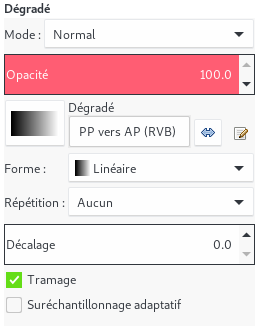
\includegraphics[width=0.3\textwidth]{Images/color_tool_2_settings.png}
	\end{center}
	Il existe de nombreux modes et de nombreuses formes, n'hésitez pas à les essayer pour les découvrir. 
	
\end{frame}




\begin{frame}
	Installation
	
	\begin{itemize}
	\item Windows
	
	\fbox{\url{https://www.gimp.org/downloads/}}
	
	\item Linux
	
	%\begin{lstlisting}[language=bash]
  	%$ sudo apt install gimp
	%\end{lstlisting}
	
	\item MAC OS X
	
	\fbox{\url{https://www.gimp.org/downloads/}}
		
	\end{itemize}
\end{frame}

\begin{frame}
	Le libre rapidement 
	
	Permet de faire plein de choses cool (et rapides)
	
	Adacity,...
\end{frame}

\begin{frame}
	
	\begin{enumerate}
	\item Ouvrir une image : File/open ==> choisir l'image à ouvrir 
	
	Ou ... plus simple : faire glisser l'image sur l'environnement de travail
	
	\item Créer un nouveau projet ==> format .xcf
	
	\item Pour obtenier une image en format "commun" ==> File/Export as ==> choisir le nom de fichier et l'extension (.png, .jpeg, .pdf, .text, .gif, .ps, .psd(compatibilité photoshop),...)
	\end{enumerate}
\end{frame}

\begin{frame}
	Description rapide des fenêtres 
	\begin{enumerate}
	\item Menu
	\item Fenêtre d'outils 
	\item Fenêtre de calques 
	
	\end{enumerate}
	Environement ouvert (échelles, zone de travail)
\end{frame}

\begin{frame}
	Outils : description générale
	
	Ctrl + B pour l'ouvrir (ou windows/Toolboxes)
	
	\begin{enumerate}
	\item Double clique pour les paramètres
	\end{enumerate} 
\end{frame}

\begin{frame}
	Outils : description par outil
	
	+ Raccourcis de l'outil
	
	+ Paramètres les plus courraments utilisés
\end{frame}

\begin{frame}
	Crayon
	
	Majuscule maintenue + Clique ==> tracer une ligne droite 
\end{frame}

\begin{frame}
	Layer manager 
	
	Ctrl + L (ou windows/Layers) pour l'ouvrir
	
	$\Rightarrow$ pour masquer, superposer, mettre à l'avant plan,... 
	 
	\begin{itemize}
		\item Calque (tel quel)
		\item Texte 
		%\item Filtre (déconseillé)
	\end{itemize}
	
	Attention : modifications QUE sur les layers sélectionnés 
	
	+ Masque (= ...) 
	\todo[inline]{exemple photo (layes cachés,...)}	 
\end{frame}

\begin{frame}
	Selection editor (All, shrink, grow, invert,...)
	
	$\Rightarrow$ Clique droit/	Select/All,Invert,None,...
\end{frame}

\begin{frame}
	Canaux (alpha et différentes couleurs)
	
	Canal alpha = ??
	
	Opérations sur les couleurs (mentionner rapidement : niveaux, balances, seuils, saturation,...)
\end{frame}

\begin{frame}
	Filtres et effets (ombres sous le texte,...)
\end{frame}

\begin{frame}
	\todo[inline]{Exercices : .text, contourner automatiquement, texte "3D"}
\end{frame}

\appendix 

\begin{frame}
	Récapitulatif des raccourcis 
	\begin{itemize}
	%todo A CLASSER (ex: view, selection, tools, ...)
	\item Ctrl + B
	\item Ctrl + L
	\item Raccourcis classiques (Ctrl + A (tout sélectionner), MAJ + Ctrl + A (tout déselectionner), Ctrl + C, Ctrl + V, Ctrl + I (inverser la sélection)...)
	\item +
	\item -
	\item 1,2,3,4,5, MAJ + 2, MAJ + 3, MAJ + 4, MAJ + 5  
	\item R = rectangle 
	\item E = ellipse 
	\item F = free select
	\item Ctrl appuyé = sélection de couleur
	\end{itemize}
	
	\url{http://www.gimpusers.com/gimp/hotkeys}
\end{frame}

\begin{frame}
	Tutoriels gimp bien foutus
	\url{https://docs.gimp.org/fr/}
\end{frame}

\begin{frame}
	G'MIC
\end{frame}
\end{document}
